\chapter{روش انجام پروژه}
\section{مقدمه}

برای اجرای این پروژه راه‌های متفاوتی مورد بررسی قرار داده شد تا بتوان بهترین آنها را روی پهپاد پیاده‌سازی کرد. نتیجه نهایی پیاده سازی ۳ شبکه کانولوشن
به صورت پی در پی است. شبکه اول برای آشکارسازی موقعیت کف دست است. بدین صورت که هر فریم گرفته‌شده از دوربین پهپاد 
پس از تغییر اندازه به یک ماتریس ددد*پپپپ*۳ به ورودی مدل داده می‌شود و پس از پردازش آن خروجی یک ماتریس ۲۵۶*۲۵۶*۳ است که جعبه محدودکننده 
دست را شامل می‌شود. پس از آن، این ماتریس به مدل دوم به عنوان ورودی داده می‌شود، در این مدل جعبه مرزی برش خورده دست به صورت یک ماتریس گرفته‌شده و خروجی آن برابر ۲۱ نقطه 
سه بعدی عطف دست و شاخص دست(راست یا چپ) است.  در ادامه مدل سوم به عنوان ورودی، یک ماتریس ۲۱*۲ می‌گیرد که مختصات نقاط  طول و عرض هر نقطه عطف دست است س=
چرا که عمق تصویر با توجه به ژست‌های در نظر گرفته شده از اهمیت بالایی برخوردار نیست. و در خروجی پیش‌بینی می‌کند که کدام ژست دست مد نظر کاربر است. با توجه به این پروژه ۹ ژست 
گوناگون مدنظر قرار گرفته‌شده (کاربر می‌تواند ژست‌های جدیدی اضافه کند)، خروجی شبکه کانولوشن شامل ۱۰ کلاس 
کلاس است که ۹ کلاس برای ژست‌ها و کلاسی برای زمانی که هیچ کدام از ژست‌ها انتخاب نشده در نظر گرفته‌شده.

\begin{figure}[h]
    \centering
    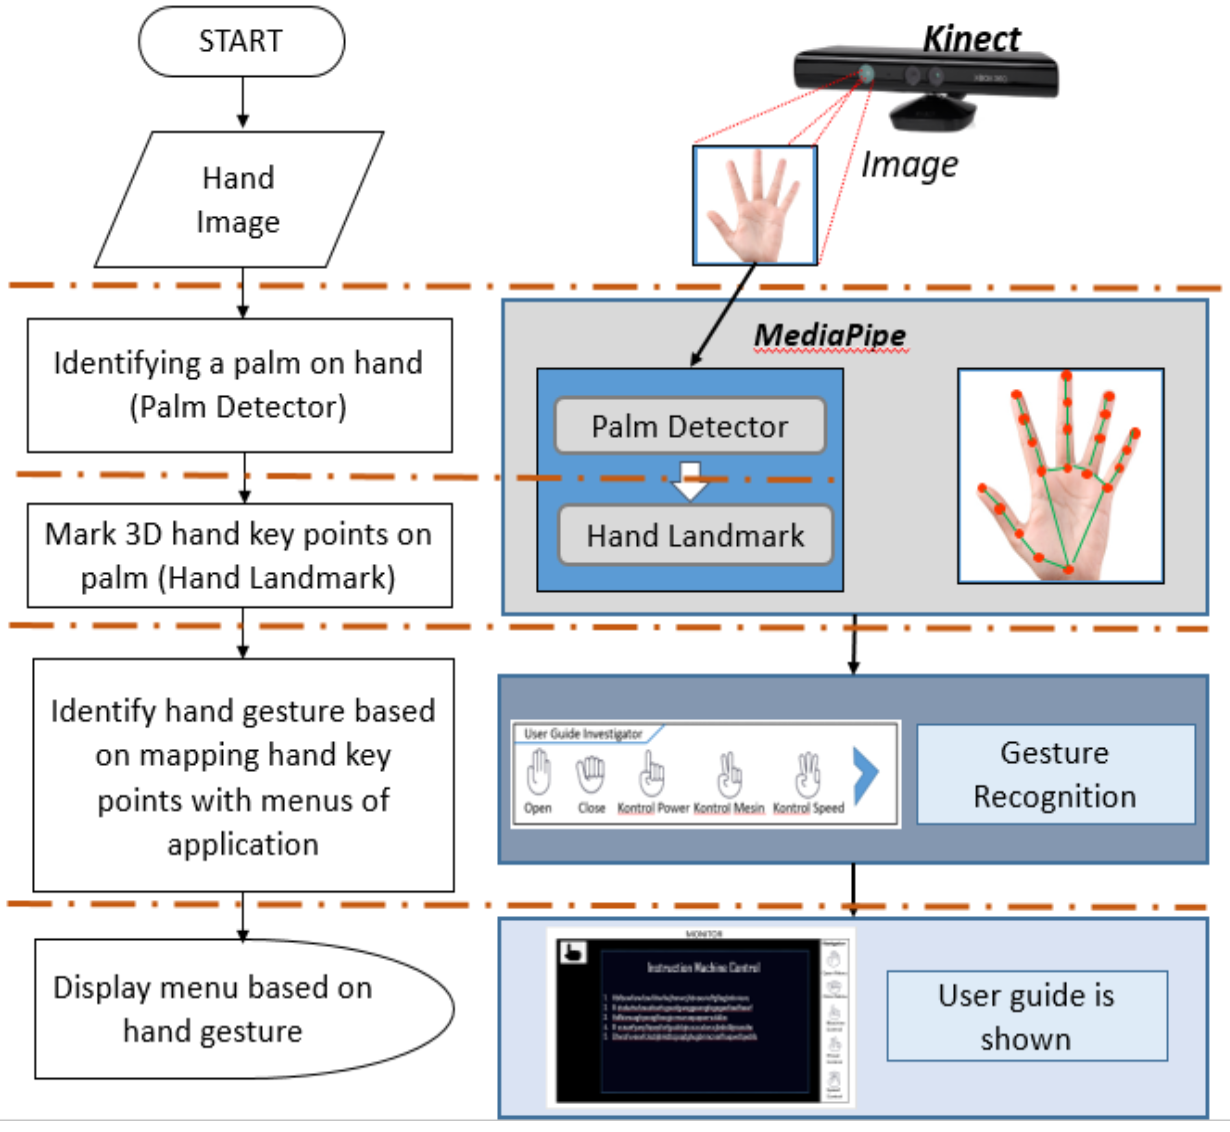
\includegraphics[width=0.7\textwidth]{gesture.png}
    \caption{تشخیص ژست دست با کمک نقاط کلیدی دست}
    % \label{test}
\end{figure}


\section{انتخاب ژست‌های دست متناسب با حرکت پهپاد}
انتخاب ژست‌های مناسب برای هر یک از حرکات پهپاد از اهمیت ویژه‌ای برخوردار است. چرا که ژست‌هایی که از لحاظ مفهومی به عملکرد پهپاد شبیه هستند راحت‌تر به خاطر سپرده شده و تجربه دلپذیرتری را در کاربر به وجود می‌آورند. 
ما برای این پروژه 9 ژست دست را در نظر گرفته‌ایم تا بتوان حرکات پایه پهپاد را با آنها انجام داد. این حرکات شامل: حرکت رو به جلو،  حرکت رو به عقب،حرکت به پایین، حرکت به بالا، حرکت به راست، حرکت به چپ، فرود آمدن، 
ایستادن در موقعیت کنونی و گرفتن عکس است که نمونه ژست دست آنها با توجه به حرکت پهپاد نشان داده شده است.

\begin{figure}[h]
    \centering
    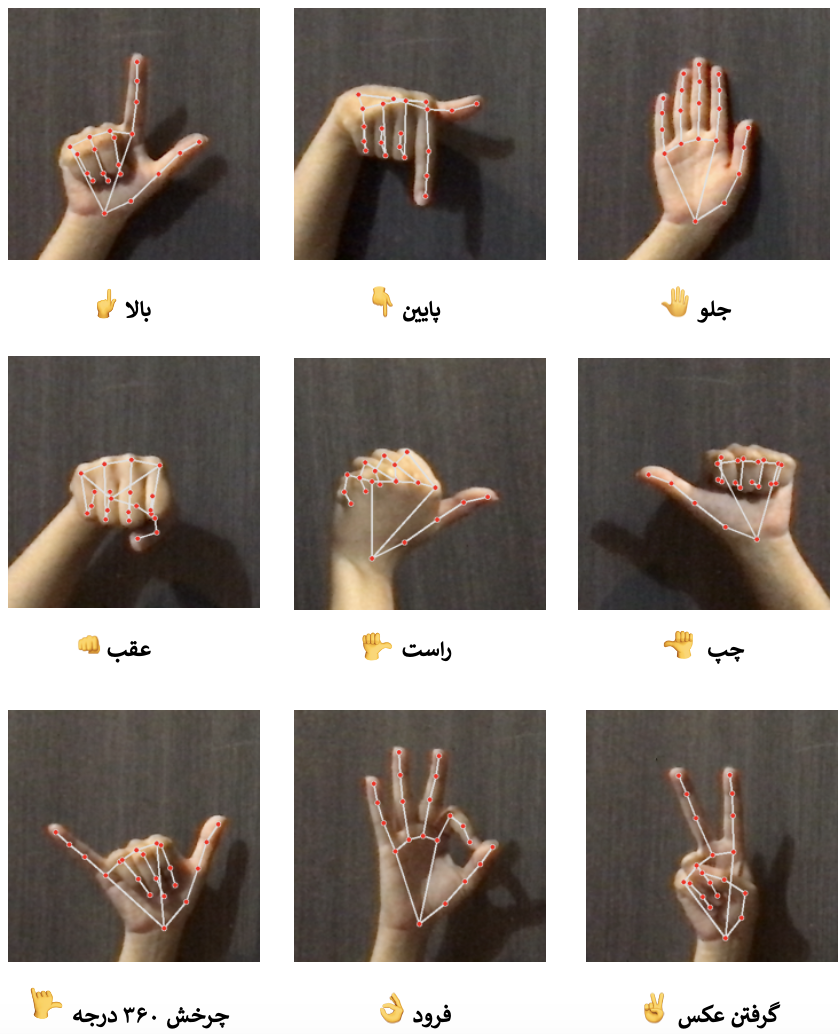
\includegraphics[width=0.7\textwidth]{gestures.png}
    \caption{نمونه‌ای از ژست‌های انتخاب‌شده در مجموعه داده‌ها}
\end{figure}

\section{دیتاست}
برای جمع آوری دیتاست مناسب پروژه، از آنجایی که ژست‌های دست را بر اساس عملکرد پهپاد تعیین کردیم تا استفاده از آنها برای کاربر مورد پسند باشند، لذا پیدا کردن دیتاست آماده ناممکن است. جمع‌آوری دیتاست مناسب و جامع از اهمیت 
بالایی برخوردار است زیرا از آنجایی که مدل باید در زمان واقعی کار کند نمی‌توان از لایه‌های زیادی استفاده کرد. پس باید برای بالا بردن دقت مدل از موارد دیگری کمک گرفت، از جمله آنها می‌توان به پیش‌پردازش، پس‌پردازش و دیتاست مناسب اشاره کرد.
از آنجایی که رویکردهای متفاوتی برای این پروژه پیاده‌سازی شد تا بتوان به بهترین راهکار برای مدلی سبک و در عین حال جامع رسید، دیتاست های گوناگونی جمع آوری شد که هر یک از آنها  ویژگی خاصی از تصویر را به عنوان دیتای 
مرود نیاز جمع‌آوری می‌کردند. از جمله ورودی کل عکس به صورت پیکسل‌های رنگی، پیدا کردن دست و ذخیره موقعیت آن به صورت پیکسل‌های 256*256، پیدا کردن نقاط کلیدی دست و ذخیره موقعیت آنها
در دیتاست و استفاده از آنها برای ورودی به مدل بهترین گزینه ممکن بود مه برای اجرای پروژه از آن استفاده کردیم.


\section{اهمیت ژست دست}
وقتی مردم صحبت می کنند، ژست می گیرند. ژست جزء اساسی زبان است که اطلاعات معنادار و منحصر به فردی را انتقال می‌دهد. ژست‌ها به گوینده کمک می‌کنند تا اهداف خود را بهتر منعکس کند. 
آن‌‌ها نقش های بسیاری را در ارتباط، یادگیری و درک هم برای افرادی که آنها را مشاهده می کنند و هم برای کسانی که آنها را ایجاد می کنند، ایفا می کنند.
وقتی مردم صحبت می کنند، دستان خود را حرکت می دهند. به حرکات خود به خودی دست که در ریتم گفتار ایجاد می شوند، حرکات هم گفتاری \LTRfootnote{co-speech gestures}
نامیده می شوند و مردم از همه فرهنگ ها و پیشینه های زبانی شناخته شده ژست می گیرند و برای ارتباط از حرکات هم گفتاری برای رساندن بهتر مفهوم خود کمک می‌گیرند.
در واقع، نوزادان قبل از اینکه اولین کلمات خود را بیان کنند، از انواع ژست‌ها استفاده می‌کنند. دست‌های ما به ما کمک می‌کنند صحبت کنیم، فکر کنیم، و به خاطر بسپاریم، گاهی دانش
منحصر به فردی را که هنوز نمی‌توان به زبان آورد، آشکار می‌کنند. به طوری که می‌توان گفت ژست‌ها اغلب به عنوان زبان گفتاری ثانویه در نظر گرفته می شود.\cite{clough2020role}
ژست‌ها به‌ویژه زمانی مؤثر هستند که مزیتی نسبت به کلمات داشته باشند. \cite{kang2016hands}
توانایی درک شکل و حرکت دست‌ها می‌تواند یک جزء حیاتی در بهبود تجربه کاربر \LTRfootnote{user experience} 
در حوزه‌ها و پلتفرم‌های مختلف فناوری باشد. درک مفهوم ژست دست در زمان واقعی برای افراد به طور طبیعی وجود دارد، یک کار بینایی 
کامپیوتری کاملاً چالش برانگیز است، زیرا دست ها اغلب خود یا یکدیگر را مسدود می کنند مانند انسداد انگشت، کف دست و لرزش دست و فاقد الگوهای کنتراست بالا هستند.\cite{zhang2020mediapipe}

\section{کنترل پهپاد}
اکثر پهپادهای تجاری موجود در بازار یا دارای کنترلرهای طراحی شده ویژه هستند، یا دارای فرستنده سیگنال اختصاصی و برنامه‌های نرم‌افزاری هستند که روی دستگاه‌های دستی کاربران 
مانند تلفن‌های همراه یا تبلت‌ها اجرا می‌شوند. در هر دو مورد، کنترل‌کننده فرمان‌هایی را با اطلاعات دقیق از طریق کانال‌های بی‌سیم مانند 
وای‌فای یا بلوتوث ارسال می‌کند. اخیراً محصولات تجاری وجود داشته است که حرکات دست را به عنوان یک مکانیسم کنترل قابل اجرا معرفی می کنند. برای گرفتن ژست ها، دو رویکرد وجود دارد.
\begin{itemize}
    \item	استفاده از دستکش های طراحی شده ویژه: کنترل کننده بر روی دستکشی که توسط کاربران استفاده می شود نصب می شود و در زمان واقعی انحراف، گام و چرخش دست را شناسایی می کند 
    تا به حرکات مربوطه برای پهپاد را شناسایی و ارسال کند. محصولات عبارتند از \lr{Kd Interactive Aura Drone} و \lr{MenKind Motion Control Drone}
    \item 	استفاده از بینایی کامپیوتر از طریق دوربین: این دستگاه‌ها از دوربین نصب شده روی پهپاد استفاده می‌کنند تا بتوانند در لحظه تشخیص دهند که دست کاربر کجاست
    و در چه حالتی قرار دارد تا پهپاد را کنترل کند. محصولات عبارتند از \lr{DJI Spark Drone} 
\end{itemize}



\section{ابزار ها و نرم افزار های مورد استفاده}
برای پیاده‌سازی این پروژه از ابزار‌ها، نرم‌افزار‌ها و گتابخانه‌های گوناگونی استفاده شده‌است که در ادامه به توضیح دقیق آنها می‌پردازیم. قابل ذکر است که از کتابخانه‌هایی از جمله \lr{csv}، \lr{copy}، \lr{itertools} و \lr{os} نیز در قسمت‌هایی از پروژه به‌کار برده‌شده که به دلیل استفاده جزئی توضیح داده نشده.

\subsection{زبان برنامه‌نویسی پایتون}

% \subsection{کتابخانه \lr{TensorFlow}}
\lr{TensorFlow} 
\lr{TensorFlow} یک کتابخانه نرم‌افزاری رایگان و منبع باز برای یادگیری ماشین و هوش مصنوعی است. این کتابخانه توسط گوگل برین توسعه داده شده و می‌تواند در طیف وسیعی 
از وظایف یادگیری ماشین مورد استفاده قرار گیرد. همچنین تمرکز ویژه‌ای بر آموزش و استنتاج شبکه‌های عصبی عمیق دارد. 
\\
\lr{TensorFlow} انعطاف‌پذیری بالا دارد. می‌تواند برای انواع مختلف مدل‌های یادگیری ماشین از جمله شبکه‌های عصبی پیچشی \LTRfootnote{Convolutional neural network}، شبکه‌های عصبی بازگشتی \LTRfootnote{Recurrent neural network} و شبکه‌های مولد متخاصم \LTRfootnote{Generative adversarial network} مورد استفاده قرار گیرد.
\lr{TensorFlow} قابلیت اجرای مدل‌ها بر روی پردازنده‌های چندگانه، پردازنده‌های گرافیکی \LTRfootnote{GPU} و حتی \lr{TPU}های خاص گوگل را دارد. همچنین به دلیل محبوبیت و پشتیبانی گسترده،
منابع آموزشی و کتابخانه‌های جانبی فراوانی برای آن وجود دارد. به طور کلی،\lr{TensorFlow}  یکی از ابزارهای قدرتمند و پرکاربرد در حوزه یادگیری ماشین و هوش مصنوعی است.

\subsection{کتابخانه \lr{Scikit-learn}}
\lr{Scikit-learn} که با نام‌های \lr{scikits.learn} و \lr{sklearn} نیز شناخته می‌شود یک کتابخانه یادگیری ماشین رایگان و منبع باز برای زبان برنامه‌نویسی پایتون است. این کتابخانه شامل الگوریتم‌های مختلفی برای طبقه‌بندی،
رگرسیون و خوشه‌بندی مانند ماشین‌های بردار پشتیبان، جنگل‌های تصادفی، تقویت گرادیان، \lr{k-means} و \lr{DBSCAN} می‌باشد. \lr{Scikit-learn} به طور ویژه برای تعامل با
کتابخانه‌های \lr{NumPy} و \lr{SciPy} طراحی شده است و ابزارهای متنوعی برای پیش‌پردازش داده‌ها، انتخاب و ارزیابی مدل‌ها و کاهش ابعاد فراهم می‌کند. این کتابخانه به کاربران کمک می‌کند تا به راحتی از آن در پروژه‌های 
یادگیری ماشین خود استفاده کنند. این کتابخانه به دلیل سادگی و کارایی خود در بین محققان و مهندسان داده بسیار محبوب است و امکانات وسیعی را برای توسعه و ارزیابی مدل‌های یادگیری ماشین فراهم می‌کند.

\subsection{رابط برنامه‌نویسی \lr{Keras}}
\lr{Keras} یک رابط برنامه‌نویسی\LTRfootnote{API} یادگیری عمیق است که به زبان پایتون نوشته شده و می‌تواند بر روی \lr{JAX}،  \lr{TensorFlow}و \lr{PyTorch} اجرا شود. هدف اصلی \lr{Keras} کاهش پیچیدگی‌ها و بار شناختی توسعه‌دهندگان است، 
به طوری که آنها بتوانند روی بخش‌های حیاتی و مهم پروژه‌های یادگیری ماشین تمرکز کنند. این رابط برنامه‌نویسی با رابط کاربری ساده و کاربرپسند، امکان توسعه سریع مدل‌های پیچیده را فراهم
می‌کند. \lr{Keras} همچنین عملکرد بالایی دارد و توسط سازمان‌های بزرگی نظیر ناسا، یوتیوب و \lr{Waymo} برای تحلیل داده‌ها، بهبود الگوریتم‌های توصیه‌گر و توسعه سیستم‌های خودران مورد استفاده قرار 
می‌گیرد. این کتابخانه با مستندات جامع و پشتیبانی از جامعه کاربری بزرگ، به یکی از ابزارهای محبوب در حوزه یادگیری عمیق تبدیل شده است.

\subsection{کتابخانه‌های\lr{MediaPipe}}
\lr{MediaPipe} مجموعه ای از کتابخانه ها و ابزارهایی است که از تکنیک‌های هوش مصنوعی و یادگیری ماشین در برنامه‌های خود استفاده می‌کند.
این کتابخانه برای برنامه‌نویسان یادگیری ماشین از جمله محققان، دانشجویان و توسعه‌دهندگان نرم‌افزار، که برنامه‌های کاربردی یادگیری ماشین را پیاده‌سازی می‌کنند، نمونه‌های
اولیه فناوری را طراحی می‌کند تا بتوان پروژه‌ها را تا حد امکان ساده کرد.
برنامه‌هایی که داده‌های حسی مثل ویدیو و صدا را با نرخ فریم بالا پردازش می‌کند تا تجربه کاربر را بهتر کند. مراحل پردازش یا مدل‌های استنتاجی ممکن است دشوار باشد، چون 
گاهی اتصال بین مراحل زیاد است. همچنین، توسعه برنامه برای پلتفرم‌ زمان‌بر است. \cite{lugaresi2019mediapipe}
\\
\lr{Media Pipe} این چالش‌ها را با انتزاع و اتصال مدل‌های مختلف به یکدیگر در یک چارچوب مناسب حل می‌کند. با استفاده از \lr{MediaPipe}، می‌توان یک لوله پردازش را به صورت 
گراف از اجزای مختلف، از جمله مدل‌های استنتاجی و عملکردهای پردازش رسانه‌ای، ساخت.
همچنین این کتابخانه می‌تواند مطابق با نیازهای افراد خود سفارشی شود و در پلتفرم‌های مختلف توسعه پیدا کند \cite{harris2021applying}.
\\
در مجموعه \lr{MediaPipe} نیز از کتابخانه‌های مختلفی برای پیاده‌سازی برنامه ها استفاده می‌شود. از جمله آنها می‌توان به \lr{Tensor Flow}، \lr{PyTorch}، \lr{OpenCV}، \lr{CNTK} و \lr{MXNet} اشاره کرد. \cite{harris2021applying}

\begin{figure}[h]
    \centering
    \includegraphics[width=0.85\textwidth]{mediapipe2.png}
    \caption{برخی کاربردهای کتابخانه \lr{MediaPipe}}
\end{figure}

\subsection{کتابخانه \lr{NumPy}}
\lr{NumPy} کتابخانه‌ای برای محاسبات علمی در پایتون است که آرایه‌های چندبعدی و توابعی برای عملیات سریع روی آرایه‌ها ارائه می‌دهد. در هسته‌ی \lr{NumPy}، شیء \lr{ndarray} وجود 
دارد که آرایه‌های \lr{n}-بعدی با نوع داده‌ی همگن را در بر می‌گیرد و بسیاری از عملیات‌های ریاضی در آن انجام می‌شوند. این کتابخانه امکان انجام عملیات ریاضی پیشرفته و سایر 
عملیات‌ها روی تعداد زیادی داده را با کارایی بالا فراهم می‌کند، که با استفاده از دنباله‌های پایتون معمولی کارآمدی و کد کمتری دارند.

\subsection{کتابخانه \lr{Matplotlib}}
\lr{Matplotlib} یک کتابخانه متقابل پلتفرم \LTRfootnote{cross-platform}، برای تجسم داده ها و نمودارهای گرافیکی (هیستوگرام، نمودارهای پراکنده، نمودار میله ای و غیره) برای 
پایتون است. توسعه دهندگان همچنین می توانند از رابط‌های برنامه‌نویسی \lr{matplotlib}  برای جاسازی نمودارها در برنامه های رابط کاربری گرافیکی استفاده کنند.
\\
یک اسکریپت \lr{matplotlib} پایتون به گونه ای ساختار یافته است که چند خط کد تنها چیزی است که در بیشتر موارد برای تولید نمودار داده بصری مورد نیاز است. لایه برنامه نویسی \lr{matplotlib} دو رابط برنامه‌نویسی را پوشش می دهد:
\\
رابط برنامه‌نویسی \lr{pyplot}، که سلسله مراتبی از اشیاء کد پایتون است که در بالای آن \lr{matplotlib.pyplot} قرار دارد. و رابط برنامه‌نویسی اشیاء گرا \LTRfootnote{Object Oriented} که می تواند 
با انعطاف پذیری بیشتری نسبت به \lr{pyplot} مونتاژ شوند. این رابط برنامه‌نویسی دسترسی مستقیم به لایه های \lr{Backend Matplotlib} را فراهم می کند.

\subsection{کتابخانه \lr{OpenCV}}
\lr{OpenCV} یک کتابخانه متن باز برای بینایی کامپیوتری و یادگیری ماشین است که برای فراهم کردن زیرساخت مشترک برای برنامه‌های بینایی کامپیوتری و تسریع استفاده از ادراک ماشین در محصولات
تجاری طراحی شده است. این کتابخانه شامل بیش از 2500 الگوریتم بهینه‌سازی شده است که مجموعه جامعی از الگوریتم‌های کلاسیک و جدید بینایی کامپیوتری و یادگیری ماشین 
را فراهم می‌کند. \lr{OpenCV} به طور گسترده‌ای در شرکت‌ها، گروه‌های تحقیقاتی و نهادهای دولتی برای انجام پروژه‌های بینایی کامپیوتری و یادگیری ماشین استفاده می‌شود. این کتابخانه رابط‌های برنامه‌نویسی 
متعددی از جمله \lr{C++}، \lr{Python،} \lr{Java} و \lr{MATLAB} دارد که امکان انجام پروژه‌های بینایی با استفاده از زبان‌های برنامه‌نویسی مختلف را فراهم می‌کند.

\subsection{پهپاد \lr{DJI Tello}}
پهپاد \lr{DJI Tello} یک پهپاد کوادکوپتر کوچک و قابل برنامه‌ریزی است که برای مصارف آموزشی و تست پروتوتایپ توسط \lr{DJI} طراحی شده است. این پهپاد دارای ویژگی‌های ویژه‌ای مانند حرکات پایه‌ای کوادکوپتری و همچنین تکنولوژی 
کنترل پرواز \lr{DJI} و یک پردازنده \lr{Intel} بسیار قوی است. دوربین 5 مگاپیکسلی این پهپاد امکان ضبط ویدیو با کیفیت خوب را فراهم می‌کند. همچنین، پهپاد دارای یک سیستم موقعیت‌یابی بصری \LTRfootnote{Vision Positioning System} است که شامل 
یک دوربین و یک ماژول مادون قرمز 3 بعدی است و قادر است در فواصل 3.0 متر تا 30 متر ارتفاع کار کند .
\\
هسته پهپاد به عنوان مرکز پردازشی و کنترلی آن عمل می‌کند و از یک پردازنده \lr{Intel} قدرتمند پشتیبانی می‌کند. پهپاد \lr{DJI Tello} برای اجرای پروژه‌های هوش مصنوعی مانند تشخیص اشیاء روی پهپاد، از زبان 
برنامه‌نویسی پایتون و \lr{SDK} مربوطه پشتیبانی می‌کند. این \lr{SDK} به کاربران این امکان را می‌دهد که پروتوتایپ‌های پایه‌ای پروژه‌های خود را توسعه دهند و آن‌ها را بر روی پهپاد اجرا کنند .
\\
این پهپاد دارای باتری با جزئیات خاصیت مانند زمان پرواز و زمان شارژ است که می‌تواند از نظر عملکرد و ماندگاری باتری نسبت به پهپاد‌های دیگر مزیت داشته باشد. همچنین، پروژه‌های هوش مصنوعی که روی پهپاد \lr{DJI Tello} پیاده‌سازی می‌شوند، 
می‌توانند شامل تشخیص اشیاء، پیش‌بینی حرکت‌ها و یا حتی خودکارسازی فرآیندهای پروازی باشند. از جمله مدل‌های هوش مصنوعی که می‌تواند روی پهپاد \lr{DJI Tello} پیاده‌سازی شود، می‌توان به \lr{YOLOv3} اشاره کرد که برای تشخیص اشیاء با دقت بالا استفاده می‌شود.
\cite{bhujbal2022custom}

\begin{figure}[h]
    \centering
    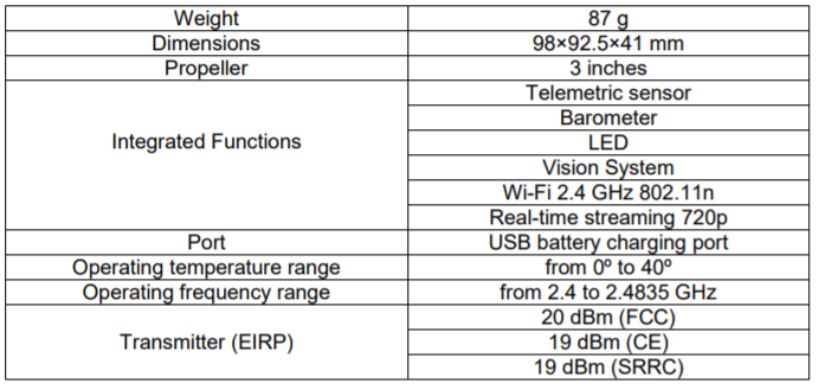
\includegraphics[width=0.7\textwidth]{table.png}
    \caption{اطلاعات پهپاد \lr{DJI Tello}}
\end{figure}




\section{مدیاپایپ}
برای پیاده سازی شبکه‌های تشخیص کف دست و پیدا کردن نقاط عطف دست از مدل‌های از قبل آموزش دیده\LTRfootnote{Pretrained} کتابخانه مدیاپایپ کمک گرفته‌شده است. مدیاپایپ  از یک خط لوله
یادگیری ماشین متشکل از چندین مدل که با هم کار می کنند استفاده می کند: یک مدل تشخیص کف دست \LTRfootnote{Palm detection model}
که تصویر را از ورودی می‌گیرد و  عکس محدوده دست را به عنوان خروجی دریافت میکند و یک مدل تشخیص نقاط عطف دست \LTRfootnote{Hand landmark model}
که عکس دست را به عنوان ورودی گرفته و مختصات‌ 21 نقطه کلیدی بند‌های انگشتان دست را در ناحیه دست تشخیص می دهد.
در عکس \ref{chart} ماژول‌های مربوط به شناسایی نقاط کلیدی نشان داده‌شده که به تفکیک هر کدام را توضیح خواهیم داد.

\begin{figure}[h]
    \centering
    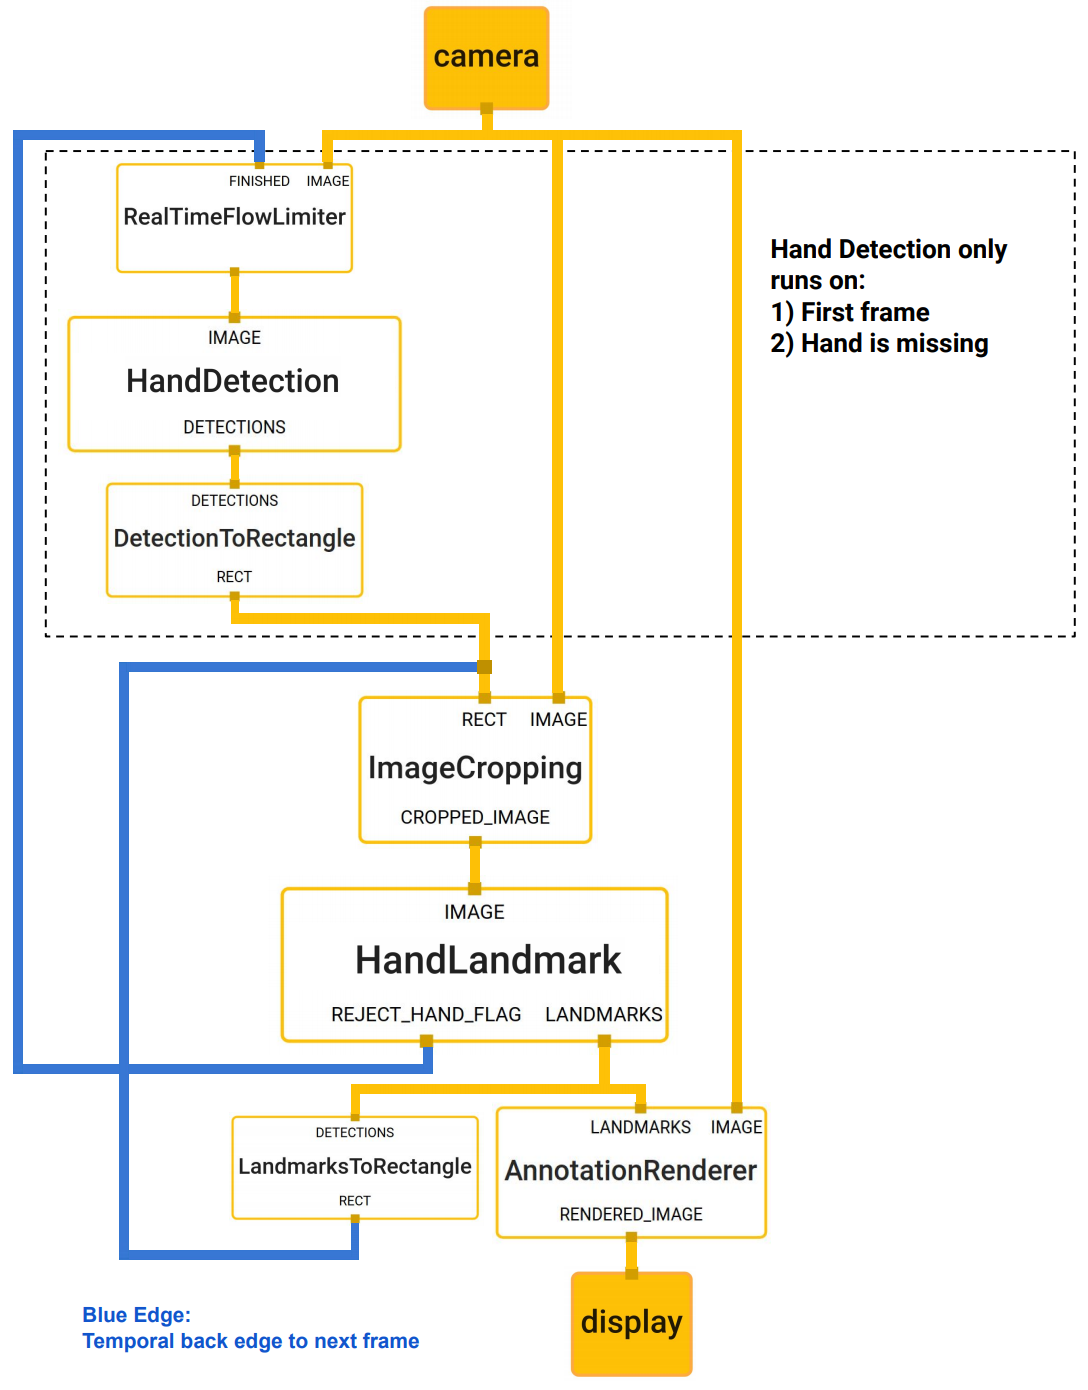
\includegraphics[width=0.7\textwidth]{hand_chart.png}
    \caption{نمودار \lr{MediaPipe} برای شناسایی نقاط کلیدی دست}
    \label{chart}
\end{figure}

\subsection{محدود کننده جریان زمان واقعی \protect\LTRfootnote{Real Time Flow Limiter}}
ماژول محدود کننده جریان زمان واقعی وظیفه محدود کردن جریان پردازش به سرعت زمان واقعی را بر عهده دارد. این ماژول امکان کنترل پردازش داده‌ها را به صورت کارآمد و در زمان واقعی فراهم می‌کند، بدون ایجاد تأخیر یا بار اضافی 
بر سیستم. ورودی‌های این ماژول شامل جریان های بسته \LTRfootnote{Packet Streams} و مهر زمان‌ها \LTRfootnote{Time stamp} می‌شود و خروجی‌های آن شامل جریان های بسته با نرخ محدود \LTRfootnote{Rate-Limited Packet Streams} و اطلاعات مربوط به 
بسته‌های حذف شده ناشی از محدودیت نرخ پردازش است. معماری این ماژول شامل مراحل بافر ورودی \LTRfootnote{Input Buffering} ، تجزیه و تحلیل مهر زمانی \LTRfootnote{Timestamp Analysis}، الگوریتم محدود کردن نرخ \LTRfootnote{Rate Limiting Algorithm}  و
بافر خروجی  \LTRfootnote{Output Buffering} است که به منظور محدود کردن نرخ جریان داده‌ها و انجام پردازش در زمان واقعی طراحی شده است. این ماژول کمک می‌کند تا بار پردازش کاهش یابد، تأخیر کاهش یابد، کیفیت خدمات حفظ شود و منابع محاسباتی بهینه‌سازی شوند .

\cite{zhang2020mediapipe}



\subsection{تشخیص دست \protect\LTRfootnote{Hand Detection}}
ماژول تشخیص کف دست که یکی از دو ماژول اصلی است، در مدیاپایپ دارای دقت متوسط 95.7 درصد است که این دقت بالا با استفاده از استراتژی‌های مختلف به دست آمده است. این ماژول از یک مدل تشخیص کف دست استفاده می‌کند 
به جای تشخیص دست، زیرا تشخیص محدوده‌های اجسام سفت و سخت مانند کف دست و مشت بسیار ساده‌تر از تشخیص دست‌ها با انگشتان مفصلی است. از الگوریتم سرکوب غیر حداکثری برای حذف تشخیص‌های تکراری و انتخاب 
مرتبط‌ترین اشیاء شناسایی شده استفاده می‌شود که به کاهش مثبت کاذب و پیچیدگی محاسباتی کمک می‌کند. وظیفه اصلی این ماژول تشخیص دست در تصویر و محاسبه مکان دقیق دست است. این ماژول برای تشخیص دست در تصویر و 
محاسبه مکان دقیق دست استفاده می‌شود و پس از تشخیص دست، مکان دقیق دست را به ماژول‌های بعدی ارسال می‌کند.
\\
ماژول تشخیص دست در مدیاپایپ یکی از ابزارهای کلیدی برای تشخیص دست‌ها در تصاویر و ویدیوها است. این ماژول قادر است به‌صورت دقیق و کارآمد موقعیت دست‌ها را شناسایی کند و نواحی مربوطه را برای پردازش‌های بعدی فراهم 
کند. ورودی این ماژول شامل تصویر یا فریم ویدیو و پارامترهای تنظیمات است، در حالی که خروجی آن شامل مستطیل‌های محدوده دست‌ها، نمرات اطمینان و در صورت فعال بودن، دست غالب \LTRfootnote{handedness} است. معماری این 
ماژول شامل مراحل پیش پردازش  \LTRfootnote{Preprocessing}، مدل تشخیص دست و پس پردازش \LTRfootnote{Postprocessing}  است که به ترتیب شامل نرمال‌سازی و تغییر اندازه تصویر، شبکه عصبی تشخیص دست و فیلترینگ و محاسبه نواحی مستطیلی دست‌ها می‌باشد.
\\
وظیفه اصلی ماژول شناسایی و محصور کردن دست‌ها در تصاویر و ویدیوها است که در کاربردهای مختلفی از جمله تشخیص حرکات دست، رابط‌های کاربری بدون لمس، تحلیل رفتار و ژست‌ها و کمک به افراد کم‌توان اهمیت دارد. این 
ماژول به توسعه‌دهندگان این امکان را می‌دهد که به راحتی و با دقت بالا دست‌ها را در تصاویر و ویدیوها شناسایی کرده و از این اطلاعات برای پردازش‌های بعدی استفاده کنند.


\begin{figure}[h]
    \centering
    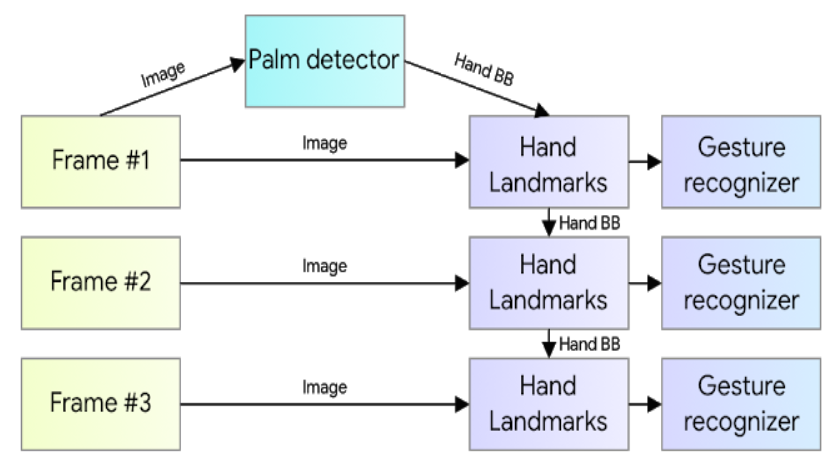
\includegraphics[width=0.7\textwidth]{mediapipe.png}
    \caption{خط لوله تشخیص دست}
\end{figure}

\begin{figure}[h]
    \centering
    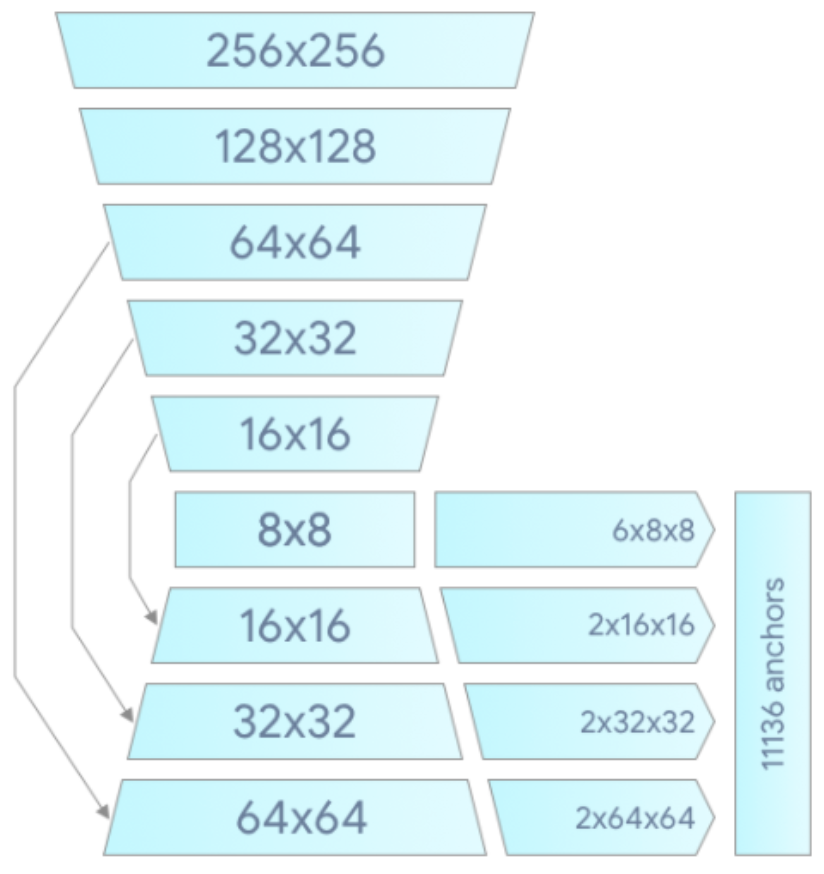
\includegraphics[width=0.4\textwidth]{hand_detector.png}
    \caption{معماری مدل آشکارساز کف دست}
\end{figure}


\subsection{تشخیص به مستطیل \protect\LTRfootnote{Detection To Rectangle}}
این ماژول وظیفه تبدیل نتایج تشخیص اشیاء به مستطیل‌های محدودکننده دست دارد. این ماژول ورودی‌هایی مانند تشخیص پروتوی \LTRfootnote{Detection Proto} و فریم تصویر \LTRfootnote{Image Frame} را دریافت کرده و مستطیل‌های محدودکننده را به صورت 
نرمال‌سازی شده و یا مطلق برای نواحی تشخیص داده شده تولید می‌کند. معماری این ماژول شامل مراحل  پیش‌پردازش، تبدیل تشخیص  \LTRfootnote{Detection Conversion} و پس‌پردازش است. وظیفه اصلی این ماژول تبدیل نتایج تشخیص به 
مستطیل‌های محدودکننده است که در کاربردهای مختلف مانند تشخیص و ردیابی چهره، تشخیص دست، امنیتی و واقعیت افزوده کاربرد دارد .
\cite{zhang2020mediapipe}

\begin{figure}[h]
    \centering
    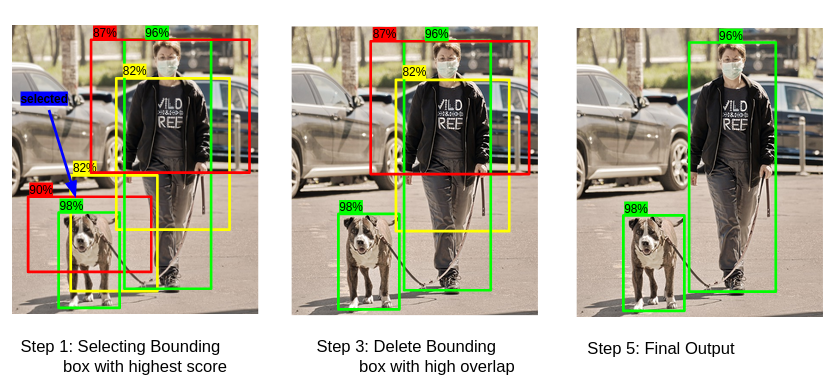
\includegraphics[width=0.55\textwidth]{bounding_box.jpeg}
    \caption{پیدا کردن مستطیل حاوی دست}
\end{figure}

\subsection{برش تصویر \protect\LTRfootnote{Image Cropping}}
ماژول برش تصویر برای برش و استخراج ناحیه‌های مورد نظر از تصاویر استفاده می‌شود. این ماژول ورودی‌هایی مانند تصویر اصلی و جعبه مرزی \LTRfootnote{bounding box} یا مختصات برش را می‌پذیرد و تصویر برش‌خورده حاوی ناحیه مورد 
نظر را تولید می‌کند. معماری این ماژول شامل مراحل پیش‌پردازش، عملیات برش\LTRfootnote{Cropping Operation}  و پس‌ پردازش  می‌باشد. وظیفه اصلی این ماژول برش دقیق ناحیه‌های مورد نظر از تصویر اصلی است که در کاربردهای 
مختلفی مانند پیش‌پردازش برای تشخیص چهره یا دست، تحلیل تصاویر پزشکی، واقعیت افزوده و پردازش تصویر در کاربردهای امنیتی مورد استفاده قرار می‌گیرد. این ماژول به 
توسعه‌دهندگان این امکان را می‌دهد که ناحیه‌های خاصی از تصاویر را به‌صورت دقیق و مؤثر استخراج کرده و برای پردازش‌های بعدی آماده کنند.
\cite{zhang2020mediapipe}

\subsection{تشخیص نقاط عطف دست \protect\LTRfootnote{Hand Landmark}}
این ماژول که دیگر اصلی است،  یک ابزار قدرتمند برای تشخیص و ردیابی نقاط کلیدی دست است. این ماژول وظیفه تشخیص و محاسبه نقاط عطف دست را بر عهده دارد. ورودی این ماژول یک تصویر است که شامل دست یا دست‌هایی 
است که می‌خواهیم نقاط کلیدی آن‌ها را تشخیص دهیم. این تصویر باید از پیش‌پردازش شده و دارای ناحیه‌ای باشد که دست در آن قرار دارد  (جعبه مرزی) که توسط ماژول دیگری مانند تشخیص دست مشخص شده است.
\\
خروجی این ماژول شامل موقعیت سه‌بعدی ۲۱ نقطه کلیدی دست است که شامل مفاصل انگشتان و نوک انگشتان می‌باشد. این نقاط کلیدی به صورت مجموعه‌ای از مختصات (\lr{x, y, z}) ارائه می‌شود 
که موقعیت هر نقطه را در فضای سه‌بعدی نشان می‌دهد و z نشان‌دهنده عمق نقطه نسبت به تصویر ورودی است.
\\
معماری این ماژول شامل استفاده از شبکه‌های عصبی عمیق برای تشخیص و ردیابی نقاط کلیدی دست است. این معماری شامل مراحل پیش‌پبردازش برای تغییر اندازه و نرمال‌سازی تصویر، تشخیص دست برای شناسایی ناحیه‌های دست، مدل 
نقاط عطف برای تشخیص دقیق نقاط کلیدی دست و پس‌ پبردازش برای تبدیل مختصات نقاط کلیدی به فرمت خروجی نهایی و اعمال اصلاحات لازم است.
\\
وظیفه اصلی این ماژول تشخیص و ردیابی دقیق نقاط کلیدی دست‌ها در تصاویر و ویدیوها است. این قابلیت می‌تواند در برنامه‌های مختلفی مانند واقعیت افزوده (\lr{AR})، رابط‌های کاربری بدون لمس،
تحلیل حرکات، تشخیص حرکات دست در زبان اشاره و ... استفاده شود و توسعه‌دهندگان را قادر می‌سازد از این قابلیت‌های پیشرفته در برنامه‌های خود بهره ببرند.
\cite{zhang2020mediapipe}


\begin{figure}[h]
    \centering
    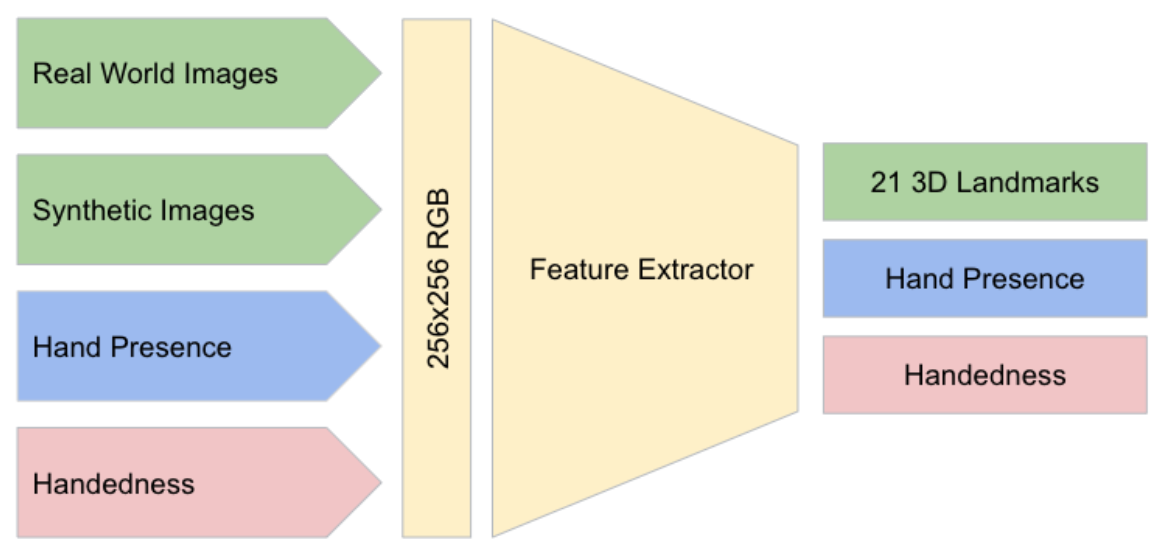
\includegraphics[width=0.7\textwidth]{landmark.png}
    \caption{معماری مدل نقطه عطف دست. این مدل دارای سه خروجی است که یک استخراج کننده ویژگی را به اشتراک می گذارند. هر سر توسط مجموعه داده های مربوطه که با همان رنگ مشخص شده اند آموزش داده می شود.}
\end{figure}

\begin{figure}[h]
    \centering
    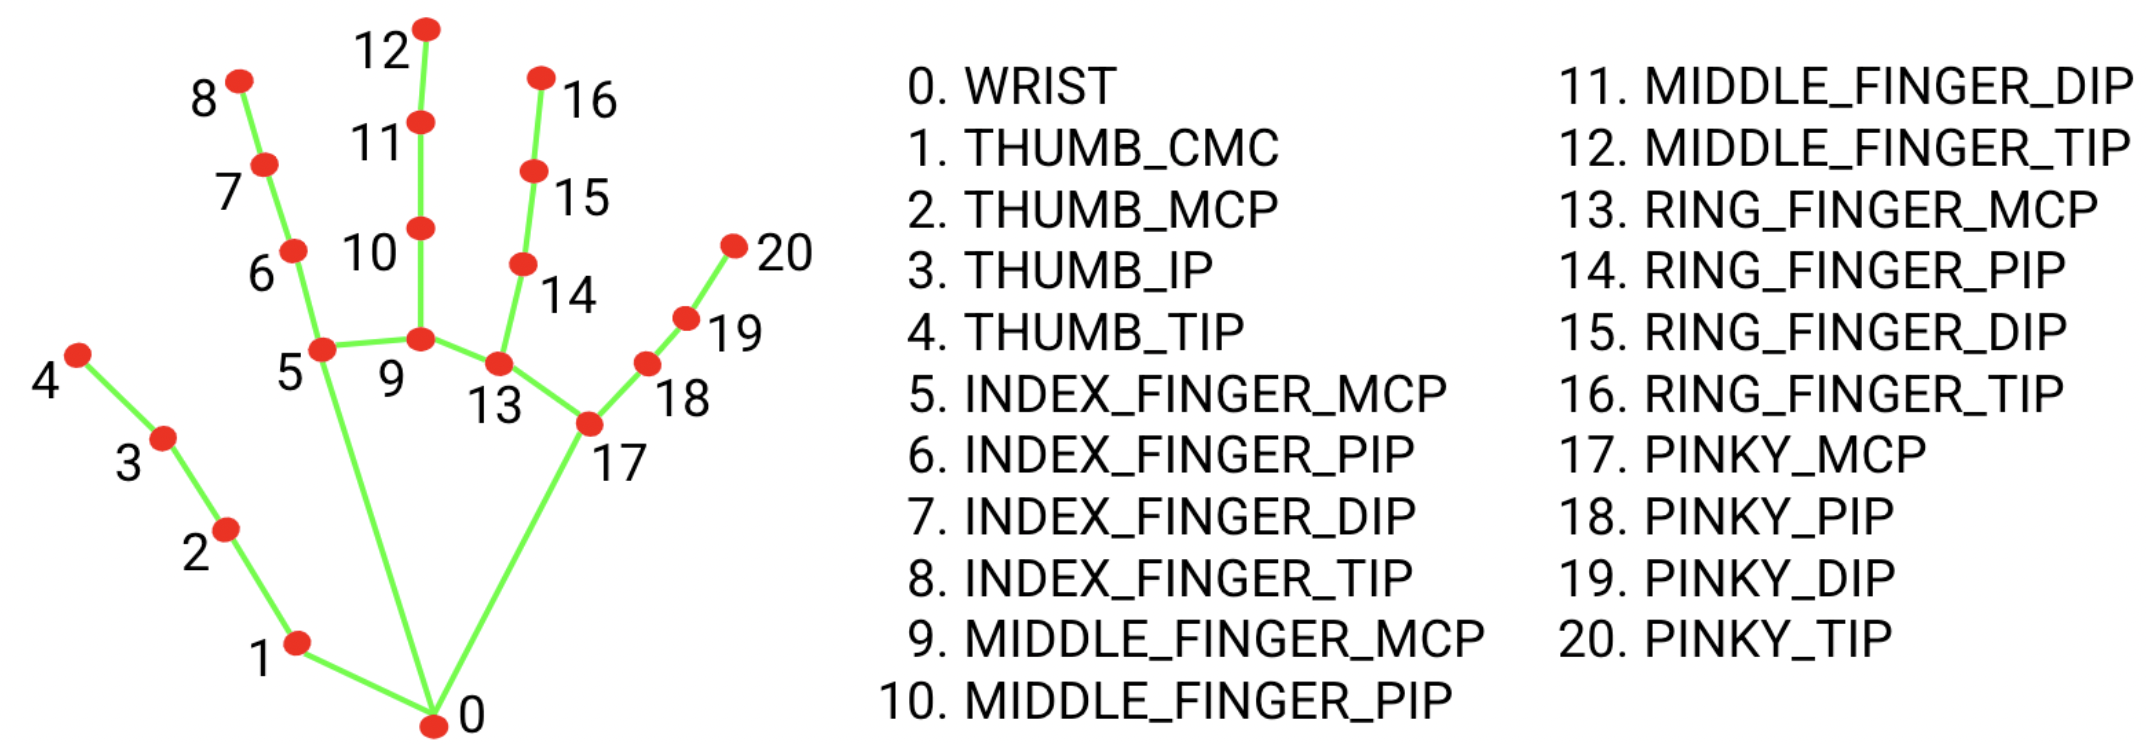
\includegraphics[width=1\textwidth]{hand-landmarks.png}
    \caption{موقعیت ۲۱ نقطه کلیدی در ناحیه دست}
\end{figure}



\subsection{نقاط عطف یه مستطیل \protect\LTRfootnote{Landmarks To Rectangle}}
این ماژول برای تبدیل نقاط کلیدی به مستطیل‌های محدودکننده استفاده می‌شود. این ماژول وظیفه دقیق محصور کردن نقاط کلیدی یک شیء، مانند دست یا چهره، را بر عهده دارد. با استفاده از این مستطیل‌ها، می‌توان موقعیت دقیق‌تر اشیاء در 
تصویر را نمایش داد و از آن‌ها به عنوان ورودی برای ماژول‌های بعدی در گراف استفاده کرد. این ماژول شامل مراحل پیش‌پردازش داده‌های ورودی، محاسبه مستطیل محدودکننده، نرمال‌سازی مختصات مستطیل‌ها و تولید خروجی نهایی 
می‌باشد. وظیفه اصلی این ماژول تبدیل نقاط کلیدی به مستطیل‌های محدودکننده دقیق است که در بسیاری از کاربردها اهمیت دارد، از جمله ردیابی اشیاء، تحلیل حرکات، پیش‌پردازش برای مدل‌های دیگر و افزایش دقت در پردازش تصویر .
\cite{zhang2020mediapipe}


\subsection{ارائه کننده حاشیه نویسی \protect\LTRfootnote{AnnotationRenderer}}
این ماژول برای نمایش گرافیکی نتایج پردازش‌های مختلف بر روی تصاویر یا ویدیوها استفاده می‌شود. این ماژول اطلاعات حاشیه‌نویسی شامل نقاط کلیدی، مستطیل‌های محدودکننده، خطوط، متن و سایر اشکال گرافیکی را به صورت 
بصری بر روی تصاویر نمایش می‌دهد. وظیفه اصلی این ماژول شامل نمایش بصری نقاط کلیدی، مستطیل‌های محدودکننده، خطوط و اتصالات، متن و توضیحات بر روی تصاویر یا ویدیوها است. این ماژول به توسعه‌دهندگان امکان 
می‌دهد تا به راحتی و به صورت بصری نتایج پردازش‌های خود را مشاهده کنند و از این طریق به بهبود و ارزیابی عملکرد مدل‌ها و الگوریتم‌های خود بپردازند .
\cite{zhang2020mediapipe}

\subsection{مزیت‌های استفاده از کتابخانه \lr{MediaPipe}}












\section{پیش‌پردازش}
برای ورود نقاط عطف دست به مدل تعیین ژست به ۲۱ مختصات طول و عرض نیاز داریم. خروجی مدل تعیین مختصات نقاط عطف دست برابر مختصات مطلق پیکسل ها نسبت به گوشه سمت 
چپ پایین تصویر است. این نقاط با توجه به اندازه عکس می‌توانند گسترده باشند برای مثال در یک عکس با اندازه ۲۰۴۸*۲۰۴۸ این اعداد از بین ۰ تا ۲۰۴۸ متغیر اند. 
اگر این مختصات را به صورت مستقیم به مدل تعیین ژست دست بدهیم دقت مدل برابر ۸۷ درصد خواهد بود که به میزان کافی مورد قبول نیست. برای بهبود آن باید پیش‌پردازش‌هایی بر روی داده ورودی انجام شود. 
\\
از جمله این پیش‌پردازش‌ها می‌توان به نسبی کردن و نرمال‌سازی داده‌ها اشاره کرد. برای این کار ابتدا باید یک مرجع واحد در نظر گرفت تا نقاط، نسبت به آن مشخص شوند. در این پروژه ما مرجع را نقطه 
مشخص شده روی مچ در نظر می‌گیریم. مختصات نقطه مرجع را برابر (0,0)  قرار می‌دهیم. سپس نسبت به آن و با توجه به فرمول زیر مختصات نقاط دیگر را به روز رسانی می‌کنیم.

% \begin{equation*}
%     X_new=\ \ (X-\ X_min)/(X_max-\ X_min)
% \end{equation*}
\[ X_{\text{\lr{rel}}} = X_{\text{\lr{ref}}} - X \]


پس از به نسبی کردن نقاط نسبت به مبدأ، آنها را با کمک فرمول زیر نرمال سازی می‌کنیم تا تمام طول و عرض نقاط به عددی میان صفر و یک به روز رسانی شوند.

\[ X_{\text{\lr{new}}} = \frac{X - X_{\text{\lr{min}}}}{X_{\text{\lr{max}}} - X_{\text{\lr{min}}}} \]
% \begin{equation*}
%     % X_new=\ \ (X-\ X_min)/(X_max-\ X_min)
% \end{equation*}

در انتها این این مختصات را به عنوان ورودی به شبکه تعیین ژست دست می‌دهیم. با توجه به اینکه معماری هیچ یک از مدل‌ها تغییر نکرد و تنها داده‌های مختصات به روز رسانی شدند، 
دقت نهایی مدل به ۹۷ درصد افزایش پیدا کرد و پیش‌پردازش تاثیر به‌سزایی در بهینه کردن پروژه داشت.


\section{رأی‌گیری پنجره‌ای}
با وجود اینکه دقت مدل پیاده‌سازی شده بالا است و عملکرد بسیار چشم‌گیری از خود نشان می‌دهد، در عین حال پیش‌بینی اشتباه مدل می‌تواند عواقب زیان‌باری را به ارمغان آورد، 
از تجربه ناپسند برای کاربر گرفته تا برخورد پهپاد به اجسام و هزینه مالی. لذا باید دقت انجام پروژه را از آنچه مدل پیش‌بینی می‌کند نیز بالاتر برد. برای این کار از رأی‌گیری پنجره‌ای 
استفاده کرده‌ایم. بدین صورت که متغیری را با توجه به \lr{FPS} دوربین در نظر می‌گیریم بدین صورت که هر چه \lr{FPS} دوربین پهپاد بیشتر باشد متغیر در نظر گرفته‌شده نیز بیشتر 
است، برای مثال در پروژه ما از آنجایی که دوربین پهپاد برابر 30 \lr{FPS} است ما این متغیر را ۱۰ قرار داده‌ایم.  سپس حد مناسبی را نیز بین صفر تا یک قرار می‌دهیم که ما در 
پروژه آن را برابر 0.7  قرار داده‌ایم. طبق این راه ما ۱۰ فریم متناوب گرفته‌شده از پهپاد را به مدل پیاده‌سازی شده می‌دهیم اما تنها در صورتی دستور پیش‌بینی شده را به پهپاد
پهپاد می‌دهیم که حد ممکن را بدست آورند. برای مثال اگر ۷ یا بیشتر از ۱۰ حرکت پیش بینی شده، دستور حرکت رو به جلو باشد آنگاه به پهپاد دستور داده می‌شود تا به جلو حرکت کند. 
در غیر این صورت اگر کمتر از ۷ عدد از فریم‌ها یک ژست دست را پیش‌بینی نکنند، پهپاد در حالت قبلی خود باقی می‌ماند و دستوری به آن داده نمی‌شود.
